\documentclass[11pt]{article}
\usepackage[utf8]{inputenc}
\usepackage[T1]{fontenc}
\usepackage[french]{babel}
\usepackage{lmodern}
\usepackage{vmargin}

\usepackage{graphicx}

\title{[LSINF1252] Système informatique : Implémentation Malloc et Free}
\author{Julian Roussieau \and Damien Vaneberck }
\date{Mars2016}

\begin{document}

\maketitle

\section{Implémentation}

\subsection{Mymalloc} L'implémentation de mymalloc se déroule en plusieurs étapes. L'appel de mymalloc se fait avec un argument de type size\_t, cet argument donne la taille voulue pour le bloc mémoire. Lors du premier appel de la méthode, la variable globale first qui représente le premier header du bloc mémoire est NULL et lors de l'exécution de la méthode, mymalloc fait appel à sbrk sur first qui étend la taille du heap en prenant comme argument le size\_t aligné sur 32 bits. Le header first a donc un bloc mémoire assigné de la taille de size\_t, les variables du header sont modifiées pour représenter la taille allouée. Une fois cela fait, le pointeur de first est retourné. Lors d'un second appel de mymalloc, on n'étend plus la taille du heap via sbrk mais la méthode parcours la taille du bloc mémoire alloué. Si un header rencontré a comme variable alloc 0, on vérifie que la taille est suffisante pour abriter la taille qu'on veut alloué. Si c'est le cas, on écrase le header par un nouveau qui représenter ce qu'on veut alloué grâce à la méthode 'insert'.Si un bloc plus petit est rencontré, on garde en mémoire la taille de ce bloc et on continue l'itération, si le/les bloc suivants ont la taille nécessaire avec le premier bloc, on les fusionne pour assigner la mémoire. Si il y a plus de taille que prévus, un header supplémentaire est créé à la fin de la taille du bloc mémoire voulu avec comme variable alloc qui est égal à 0;

\subsection{Mycalloc}
Mycalloc a la même fonction que mymalloc excepté que mycalloc initialise toutes les variables du bloc mémoire alloué à 0. Pour se faire, la méthode prend un argument size, qui est la taille du bloc mémoire qu'on veut alloué et ensuite aligne cette taille sur un multiple de 32 bits. Ensuite, elle alloue à un pointeur size\_t, un bloc mémoire de la taille de size réaligné. Si l'allocation est déroulée correctement, la valeur pointée par le pointeur vaut 0.

\subsection{Myfree}
L'implémentation de myfree se déroule de la manière suivante, quand la méthode myfree est appelée avec comme argument le pointeur à libérer. Elle recule le pointeur de 4 bytes afin de se positionner sur la structure header. Une fois sur le header, la méthode modifie la variable 'alloc' du header pour la passer à 0, indiquant ainsi que la zone prise par la header est libre d'être écrasée lors d'un prochain appel de mymalloc.

\section{Difficultés rencontrées}
Les principales difficultés rencontrées furent dans la compilation des tests unitaires.

\section{Test Unitaire}
Les tests unitaires ont porté sur plusieurs cas possible, dans le cas de malloc, nous avons testé un simple ajout à une mémoire non-occupée et un ajout dans une mémoire remplies.\\
Pour free, nous avons testé le cas d'un libération de la mémoire et d'une assignation ensuite. Nous avons aussi testé deux cas de fragmentation différent dans la mémoire.\\
Pour calloc, nous avons testé le cas quand nous assignons deux bloc à la mémoire, pour ensuite libérer le premier et faire un calloc ensuite.

\section{Performance}

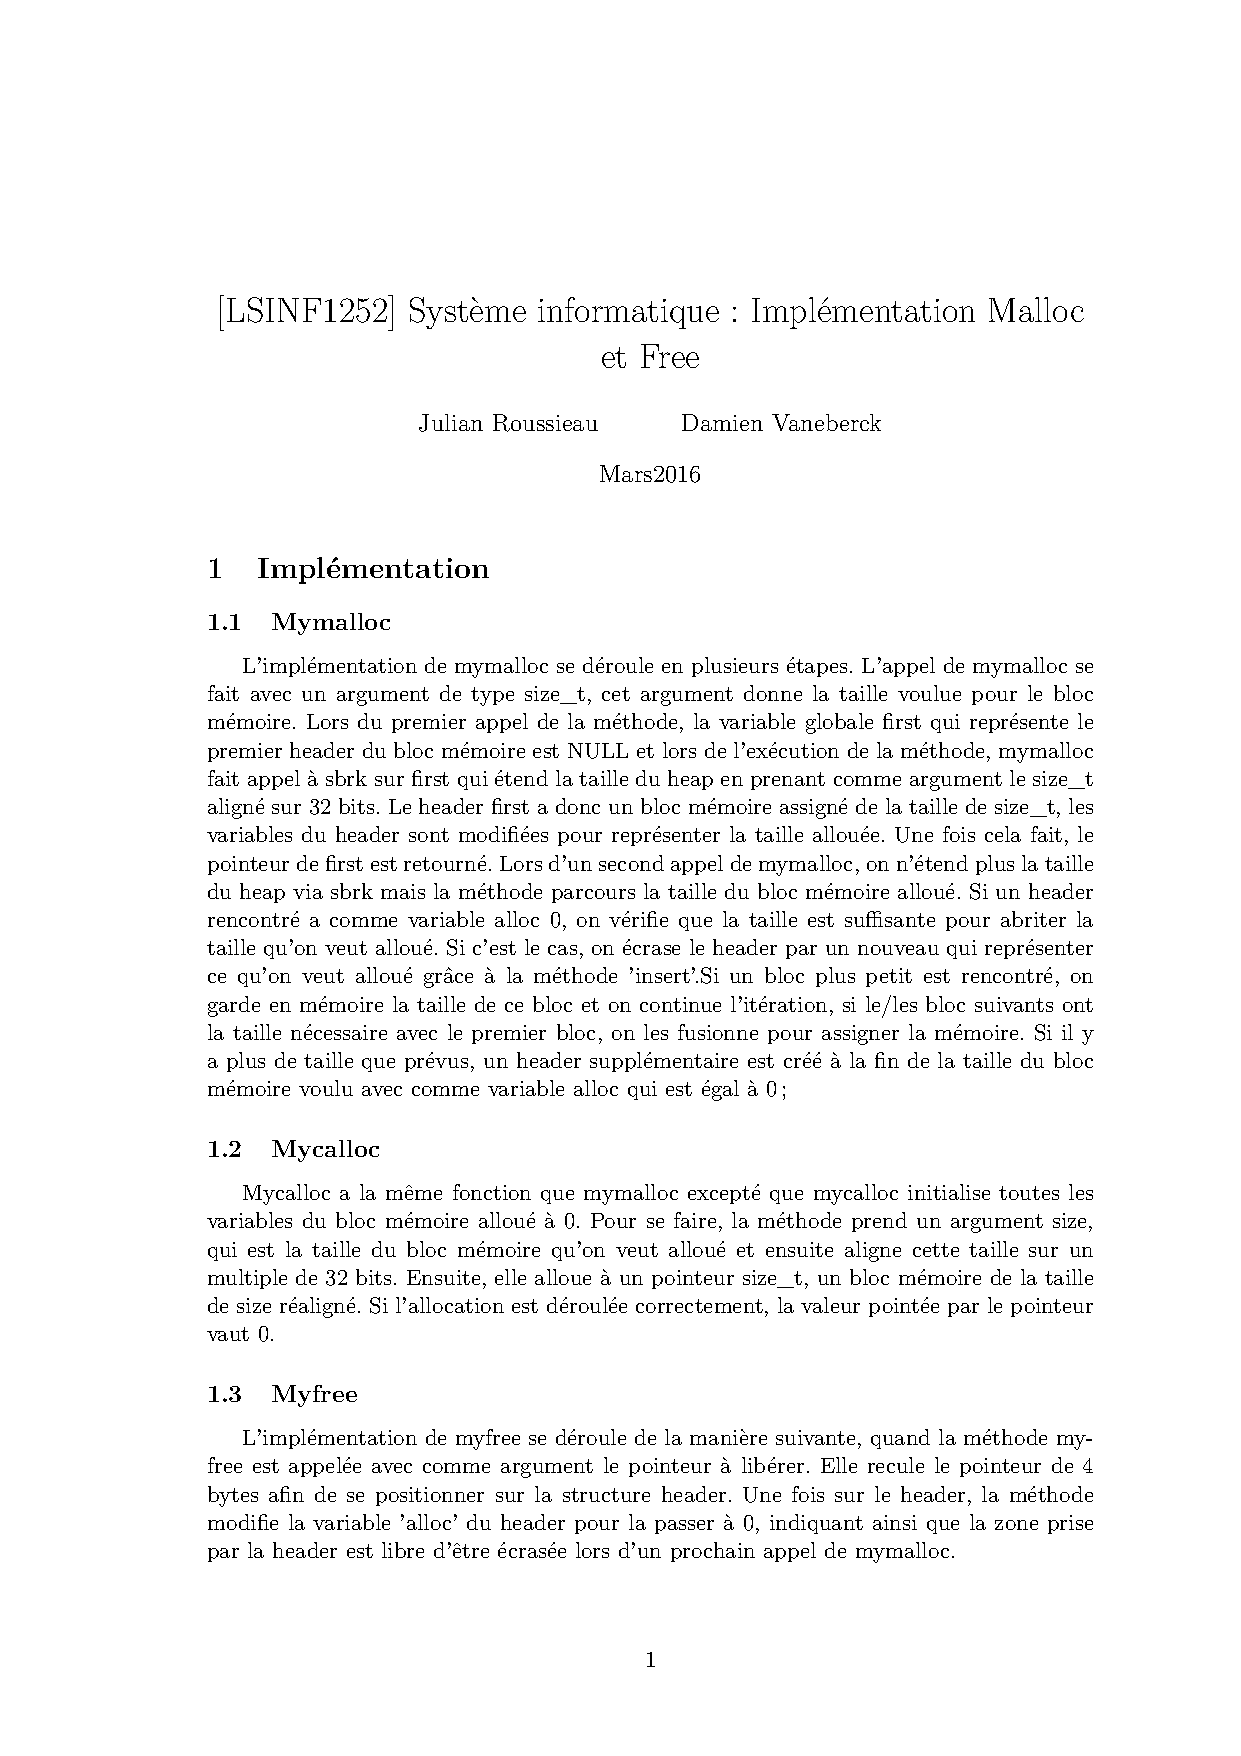
\includegraphics[width=\textwidth]{MyMalloc.png}

Nous avons ici en vert, mymalloc et en bleu, malloc. Nous pouvons voir que les deux fonctions sont linéaires. Les tests ont été effectué avec 1000,10 000,100 000,1 000 000 et 10 000 000 d'itération. Sur le graph, la fonction mymalloc est plus rapide que la fonction malloc, ce qui s'explique par la façon dont la fonction alloue une zone mémoire. Dans mymalloc, la fonction insère à la première zone mémoire libre, qu'elle soit trop grande ou non. Nous pensons que malloc, va chercher la place optimale et non la première venue.
\\
Comme nous pouvons le voir grâce au graph ci-dessus, la complexité de mymalloc est linéaire. En poussant l'analyse du code, on peut définir la complexité temporelle de mymalloc en $\mathcal{\Omega}(n)$ dans le meilleurs cas possible, c'est à dire une allocation dans une zone totalement libre. Et $\mathcal{O}(n)$ pour le pire cas. Dans un cas général, on peut dire que la complexité temporelle est en $\mathcal{O}(n)$.
\\
La complexité de free quant à elle, sa complexité aussi bien dans le pire cas que dans le meilleurs est en 1. Donc en général, on peut dire que la complexité est en $\mathcal{\theta}(1)$.
\\
Mycalloc a une complexité en O(n) car elle fait appel à mymalloc et ensuite fait une opération en temps constant, qui est l'assignation des variables à 0.

\section{Conclusion}
Implémenter malloc, calloc et free, nous a permis de mieux comprendre leurs fonctionnement ainsi que leurs utilités. Nous avons également appris à "jouer" avec les pointeurs, ce qui fait la richesse de C.
\end{document}